\documentclass{article}
\title{ECO206 Lecture Notes}
\author{Tianyu Du}
\date{\today}

% Libraries.
\usepackage{amsmath}
\usepackage{amssymb}
\usepackage{pgfplots}
\usepackage{graphicx}
\usepackage{enumitem}
\usepackage{hyperref}
\usepackage{fancyhdr}
\usepackage{perpage}
\usepackage{float}

% Property settings.
\MakePerPage{footnote}
\pagestyle{fancy}
\lhead{Notes by T.Du}
\usepackage[
	type={CC},
	modifier={by-sa},
	version={3.0},
]
{doclicense}

% Attr.
\title{ECO206 Microeconomic Theory \\ Lecture Notes}
\author{Tianyu Du}
\date{\today}
% Macro
\newcommand{\trans}[3]{{#1}: {#2} \to {#3}}
\newcommand{\R}[0]{\mathbb{R}}
\newcommand{\M}[2]{\mathbb{M}_{{#1} \times {#2}}(\mathbb{R})}
\newcommand{\coor}[2]{[\vec{{#1}}]_{{#2}}}
\newcommand{\tmat}[3]{[{#1}]_{{#2}}^{{#3}}}
\newcommand{\vset}[3]{\{\vec{{#1}_{#2}}, \dots, \vec{{#1}_{#3}}\}}
\newcommand{\sset}[3]{\{{{#1}_{#2}}, \dots, {{#1}_{#3}}\}}
\newcommand{\definition}[0]{\paragraph{Definition}}
\newcommand{\theorem}[0]{\paragraph{Theorem}}
\newcommand{\C}[0]{\mathbb{C}}
\newcommand{\restrans}[2]{{#1}\vert_{#2}}
\newcommand{\tx}[1]{\text{{#1}}}


\begin{document}
	\maketitle
	\tableofcontents
	\section{Lecture 1 May. 8 2018}
	\subsection{Budget Constraint}
	\begin{itemize}
		\item Exogenous income
		\item Endogenous income:
	\end{itemize}
	\paragraph{Bundle} Combination of goods. If we have $n$ goods, then $x_1^A$ represents a quantity ($x$) of good $1$ in bundle $A$.
	\[
		A = (x_1^A, x_2^A, \dots, x_n^A)
	\]
	
	\begin{figure*}[h]
		\centering
		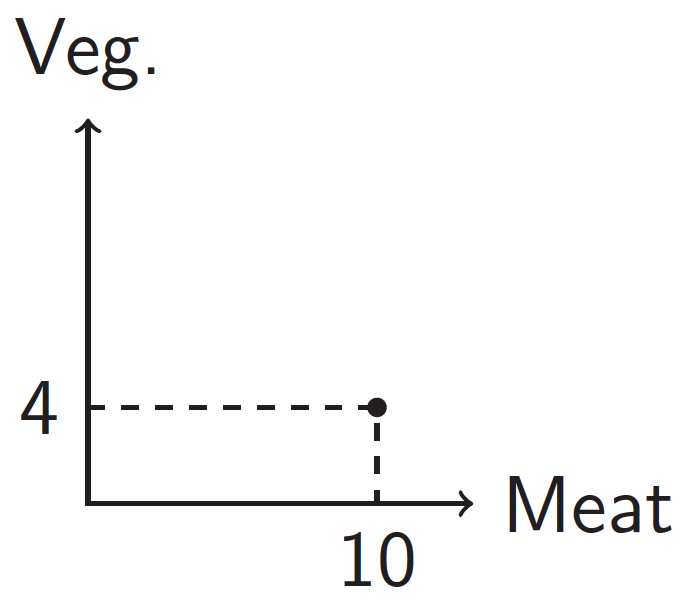
\includegraphics[width=0.3\linewidth]{eco206pic/bundle}
		\caption{Consumption bundle}
	\end{figure*}
	
	\subsubsection{Types of Income}
	\paragraph{Exogenous income}Cash(i.e. $\$$) in your pocket to spend.
	\paragraph{Endogenous income}Bundle fo goods you can sell to get money. e.g. \emph{Assets}, \emph{Skills}, \emph{Time}, etc.
	\subsubsection{Exogenous Income} Consumer walk into market with a fixed amount of \textbf{cash}, budget constraint.
	\[
	\vec{x} \cdot \vec{p} \leq I
	\]
	\begin{figure*}[h]
		\centering
		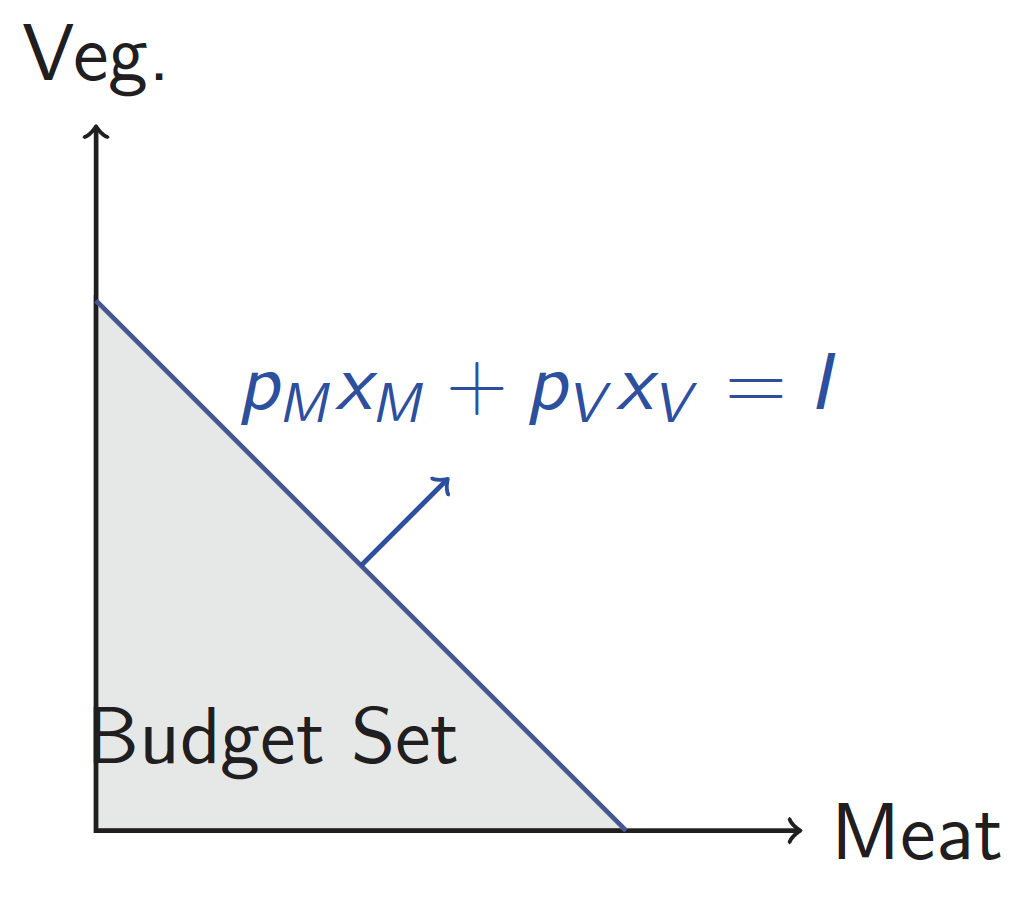
\includegraphics[width=0.3\linewidth]{eco206pic/budget}
		\caption{Budget constraint}
	\end{figure*}
	
	\subsubsection{Endogenous Income}
	\paragraph{Framework} Consumer walks into a market \textbf{without cash}, but with \textbf{endowment} $(\omega_M, \omega_V)$. And consumer can sell the endowment at market prices, the \underbar{value of the endowment} is
	\[
		p_M \omega_M + p_V \omega_V
	\]
	\paragraph{Hypothetical income} Income/Cash from selling the \emph{entire} bundle endowed. 
	\paragraph{Budget Constraint equation}
	\[
		p_M x_M + p_V x_V \leq I_{hypothetical} = p_M \omega_M + p_V \omega_V
	\]
	Intercepts: if spend all income on one good.
	\begin{itemize}
		\item x-axis(meat) = $\frac{p_M \omega_M + p_V \omega_V}{p_M} = \omega_M + \frac{p_V}{p_M}\omega_V$
		\item y-axis(veg) = $\frac{p_M \omega_M + p_V \omega_V}{p_V} = \omega_V + \frac{p_M}{p_V}\omega_M$
	\end{itemize}
	\paragraph{Assumption} consumers are price takers.
	\paragraph{Affordable} means $spending \leq income$ and $\vec{x} \in \mathbb{R}^n_{+}$
	\subsection{Opportunity Cost}
	\paragraph{OC/MRT} Rate at which one good can be traded for another though the market, \underbar{expressed in units of a good}.
	
	\emph{To get another \underbar{unit} of good 1 home many \underbar{unit} of good 2 do I need to give up?}
	\[
		\frac{dy}{dx} = -\frac{p_x}{p_y}
	\]
	\subsection{Changes that affect the budget constraint}
	\subsubsection{Pure income change} keeping relative prices constant. i.e. $\frac{p_1}{p_2} = \overline{p}$
	\begin{figure*}[h]
		\centering
		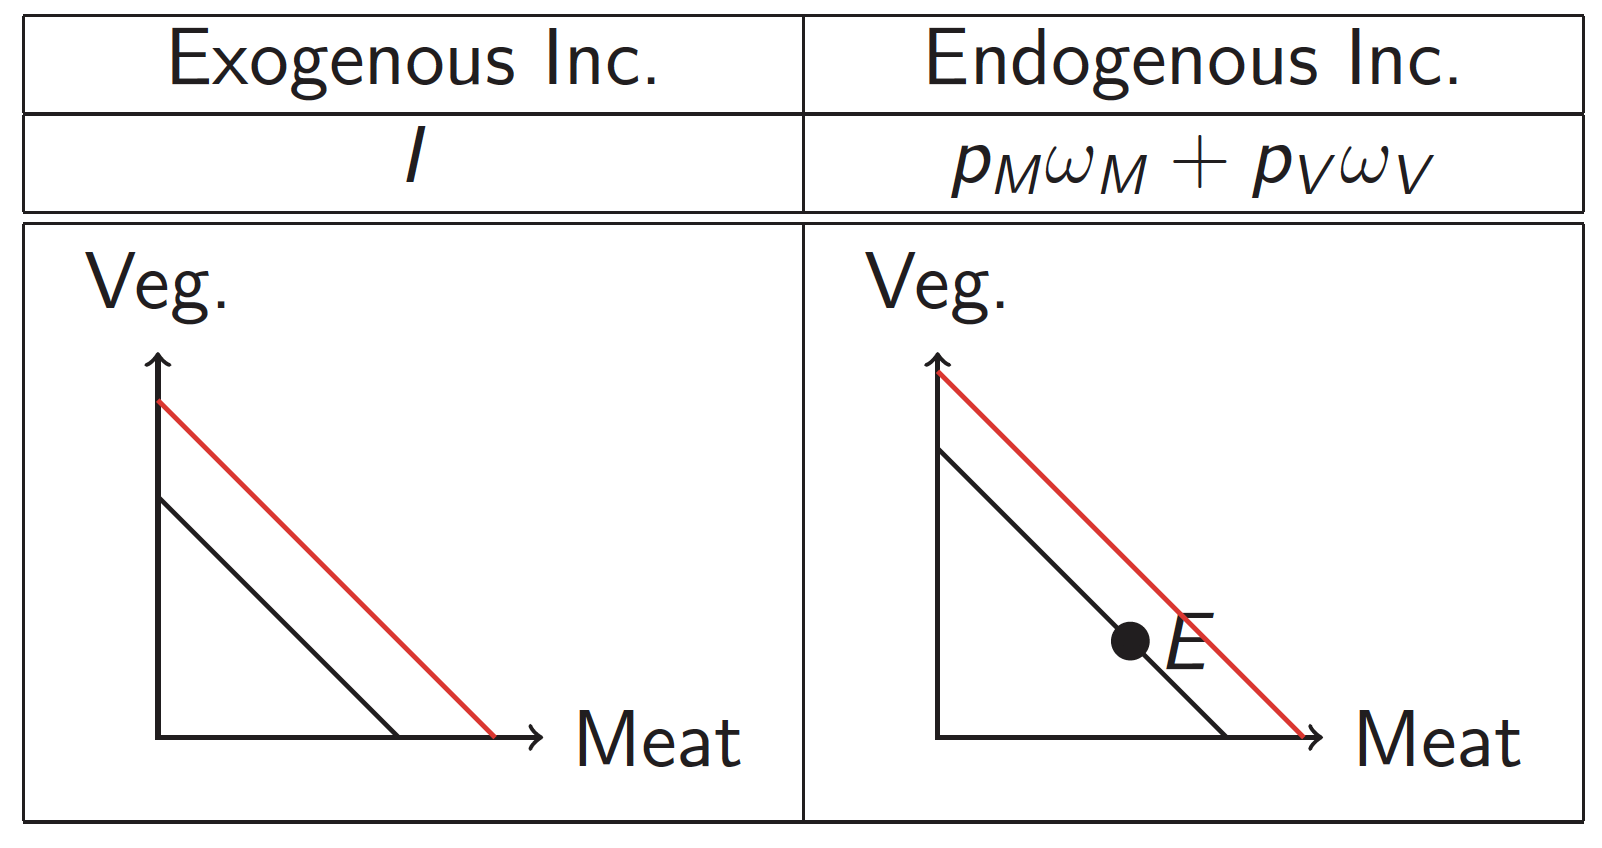
\includegraphics[width=0.5\linewidth]{eco206pic/income_change}
		\caption{Pure income change}
	\end{figure*}
	
	
	\textbf{Note} Changes in prices(relative price holds) will change the budget constraint in exogenous income budget, but will \emph{not} affect the endogenous income constraint.
	
	\textbf{Conclusion} To change budget constraint defined with endogenous income, we need \textbf{endowment changes}.
	
	\subsubsection{Price change}
	\begin{figure*}[h]
		\centering
		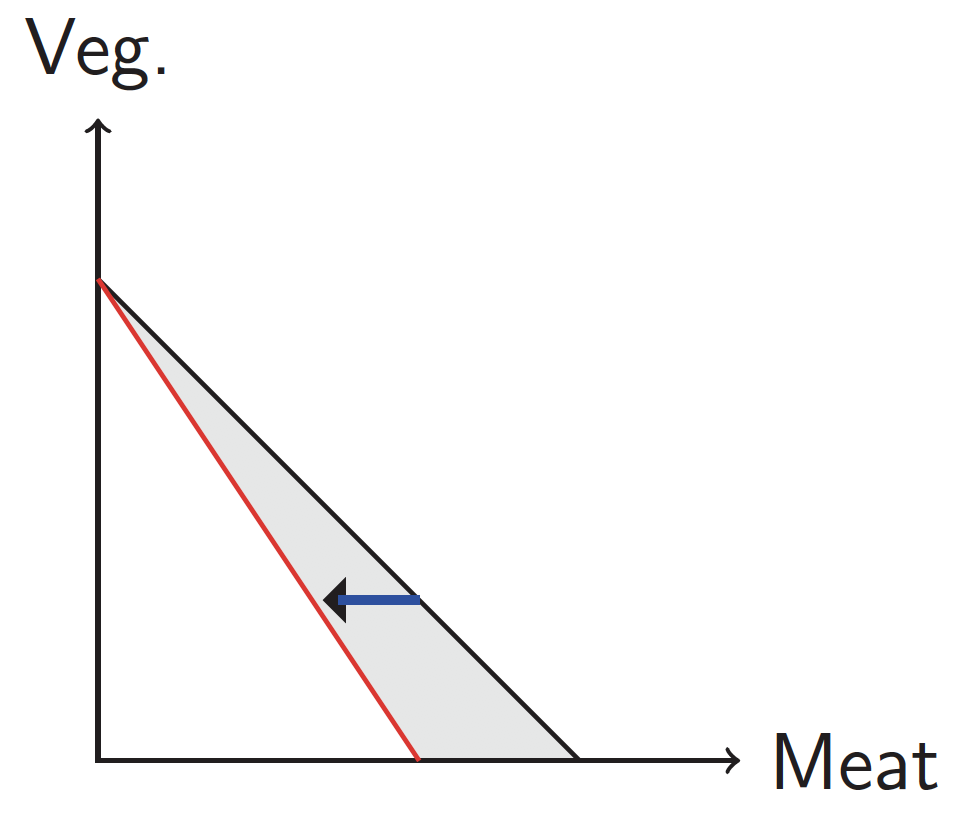
\includegraphics[width=0.5\linewidth]{eco206pic/relative_price_change}
		\caption{Relative price change}
	\end{figure*}
	
	\subsubsection{Endogenous income price change}
	\paragraph{Graph} The price of meat increases.
	\begin{figure*}[h]
		\centering
		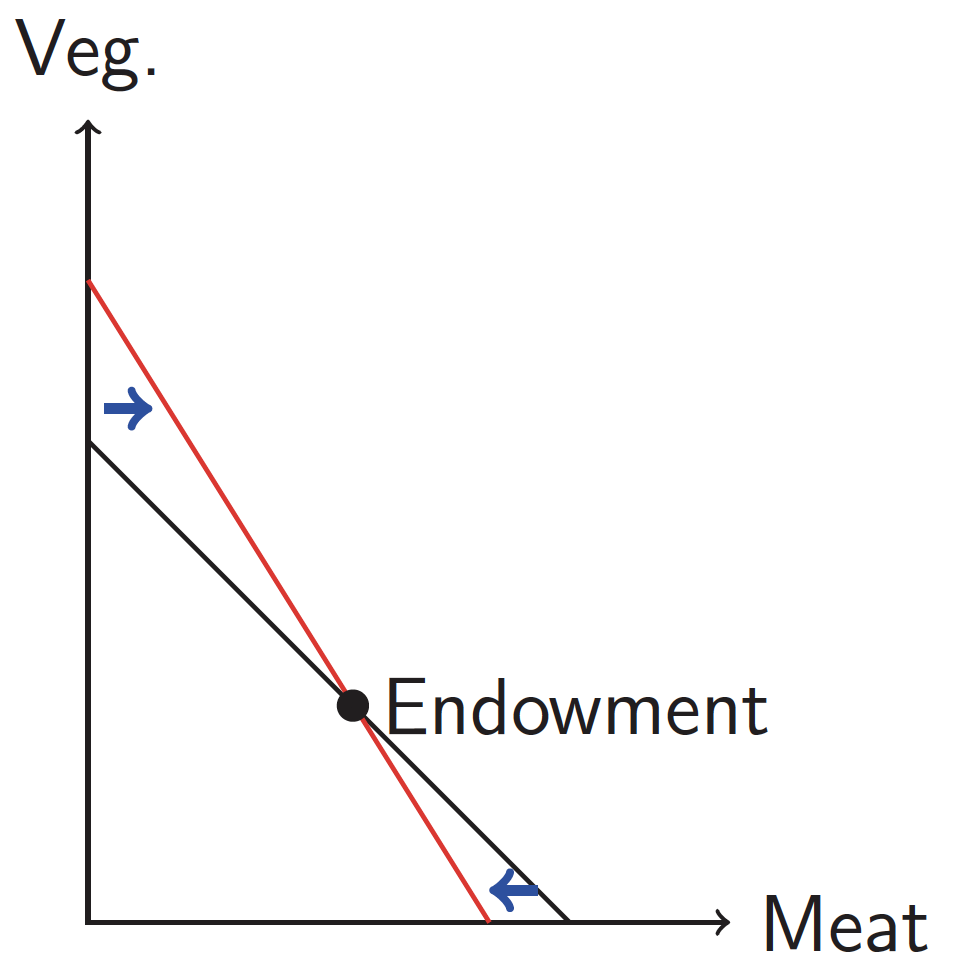
\includegraphics[width=0.5\linewidth]{eco206pic/End_price_change}
		\caption{Endogenous income price change}
	\end{figure*}
\end{document}

































